\documentclass[11pt]{article}

% ---------- Packages ----------
\usepackage[margin=1in]{geometry}
\usepackage{amsmath,amssymb,amsfonts}
\usepackage{booktabs}
\usepackage{float}
\usepackage{siunitx}
\usepackage{hyperref}
\usepackage{enumitem}
\usepackage{xcolor}
\usepackage{graphicx}
\graphicspath{{figs/}}
\hypersetup{colorlinks=true, linkcolor=blue, urlcolor=blue, citecolor=blue}
\sisetup{round-mode=places,round-precision=6,detect-weight=true,detect-inline-weight=math}

% ---------- Title ----------
\title{Gradient Descent for Linear Regression with MSE and Huber Loss\\
\large Teamwork Assignment (Learning Curves and Stop Criteria)}
\author{
  Druv Jayantilal Patel (ASU ID: 1236080380)\\
  Jay Sanjay Sonawane (ASU ID: 1233750832)\\
  Jaishva Baijubhai Patel (ASU ID: 1231581457)
}
\date{October 3, 2025}

\begin{document}
\maketitle

\begin{abstract}
We implement gradient descent (GD) for univariate linear regression under two loss functions: mean squared error (MSE) and Huber. We compare three learning rates $\eta\in\{0.01, 0.05, 0.2\}$, apply two stopping criteria (parameter-change tolerance and loss-change tolerance), and visualize efficient learning curves (one figure per loss with all $\eta$ overlaid). We validate GD (MSE) against the least-squares closed form and discuss convergence behavior and robustness.
\end{abstract}

\section{Dataset and Design Matrix}
The provided Excel sheet (\emph{Teamwork-regress w 2 losses (dataset)-1.xlsx}) supplies pairs $(x_i,y_i)$ \textit{(the same values are also provided as a CSV for convenience)}. We fit a line $\hat y = w x + b$ using the design matrix
\[
X=\begin{bmatrix}
x_1 & 1\\
\vdots & \vdots\\
x_n & 1
\end{bmatrix},\qquad
\theta=\begin{bmatrix} w\\ b \end{bmatrix}.
\]

\section{Gradient Descent Derivations}
\noindent\textit{Notation.} For MSE we set $e_i=\hat y_i-y_i$; for Huber we set $r_i=y_i-\hat y_i$. Note $e_i=-r_i$.

\subsection{MSE Loss (matches code)}
Using $e_i=\hat y_i-y_i=(wx_i+b)-y_i$, our code defines
\[
L_{\mathrm{MSE}}(\theta)=\frac{1}{n}\sum_{i=1}^n e_i^2,
\]
so the gradients are
\[
\nabla_w L_{\mathrm{MSE}}=\frac{2}{n}\sum_{i=1}^n e_i x_i,\qquad
\nabla_b L_{\mathrm{MSE}}=\frac{2}{n}\sum_{i=1}^n e_i,
\]
and GD updates are
\[
w \leftarrow w - \eta \,\frac{2}{n}\sum_i e_i x_i,\qquad
b \leftarrow b - \eta \,\frac{2}{n}\sum_i e_i.
\]

\subsection{Huber Loss}
Let $r_i=y_i-\hat y_i$ and choose $\delta>0$ (we use $\delta=0.5$). The per-sample Huber loss is
\[
\ell_\delta(r) =
\begin{cases}
\frac{1}{2}r^2,& |r|\le\delta,\\[3pt]
\delta\!\left(|r|-\frac{1}{2}\delta\right),& |r|>\delta.
\end{cases}
\]
Its derivative w.r.t.\ $r$ is
\[
\frac{\partial \ell_\delta}{\partial r}=
\begin{cases}
r,& |r|\le\delta,\\
\delta\,\mathrm{sign}(r),& |r|>\delta.
\end{cases}
\]
With $r_i=y_i-(w x_i + b)$, by chain rule $\frac{\partial r_i}{\partial w}=-x_i$ and $\frac{\partial r_i}{\partial b}=-1$, hence
\[
\nabla_w L_{\mathrm{Huber}}=-\frac{1}{n}\sum_{i=1}^n g_i x_i,\qquad
\nabla_b L_{\mathrm{Huber}}=-\frac{1}{n}\sum_{i=1}^n g_i,
\]
where $g_i=\bigl.\frac{\partial \ell_\delta}{\partial r}\bigr|_{r=r_i}$. The GD update (subtracting the gradient) becomes
\[
w \leftarrow w + \eta \,\frac{1}{n}\sum_i g_i x_i,\qquad
b \leftarrow b + \eta \,\frac{1}{n}\sum_i g_i.
\]

\section{Implementation Details}
\begin{itemize}[leftmargin=1.5em]
  \item Environment: \texttt{pandas 2.3.2}, \texttt{openpyxl 3.1.5}, \texttt{numpy}, \texttt{matplotlib}.
  \item Learning rates: $\eta\in\{0.01, 0.05, 0.2\}$.
  \item Stopping criteria:
  \begin{enumerate}[nosep]
    \item \textbf{Parameter-change tolerance} $\|\theta_{t}-\theta_{t-1}\|_2 \le \texttt{tol\_param}$ with \texttt{tol\_param} $=10^{-6}$.
    \item \textbf{Loss-change tolerance} $|L_t-L_{t-1}| \le \texttt{tol\_loss}$ with \texttt{tol\_loss} $=10^{-8}$.
  \end{enumerate}
  \item Maximum iterations: \texttt{max\_iters} $=3000$.
  \item Huber parameter: $\delta=0.5$.
  \item Validation: Compare GD(MSE) $\theta$ with least-squares solution from \texttt{np.linalg.lstsq}.
\end{itemize}

\subsection*{Termination criteria and rationale}
\begin{table}[h]
\centering
\caption{Termination criteria and thresholds}
\begin{tabular}{@{}lll@{}}
\toprule
Criterion & Definition & Value / Rationale \\
\midrule
Loss change & $|L_t-L_{t-1}|<\varepsilon_L$ & $\varepsilon_L=10^{-8}$ (objective is flat) \\
Param change & $\|\theta_t-\theta_{t-1}\|_2<\varepsilon_P$ & $\varepsilon_P=10^{-6}$ (weights stable) \\
\bottomrule
\end{tabular}
\end{table}

\section{Results}
Tables~\ref{tab:mse} and \ref{tab:huber} summarize the printed training outputs.\footnote{“stop(param)” or “stop(loss)” show which criterion triggered; “None” means the run ended via the max-iteration cap.}

\begin{table}[h]
\centering
\caption{MSE training results (updated)}
\label{tab:mse}
\begin{tabular}{@{}lcccccc@{}}
\toprule
Loss & $\eta$ & $\theta=[w,b]$ & final\_loss & stop(param) & stop(loss) & iters \\
\midrule
MSE & 0.01 & [0.7266, 0.4607] & 0.011105 & None  & None  & 3000 \\
MSE & 0.05 & [0.7333, 0.4575] & 0.011101 & \textbf{1172} & \textbf{721} & 1173 \\
MSE & 0.20 & [0.7334, 0.4575] & 0.011101 & \textbf{340}  & \textbf{204} & 341 \\
\bottomrule
\end{tabular}
\end{table}

\begin{table}[h]
\centering
\caption{Huber training results ($\delta=0.5$; updated)}
\label{tab:huber}
\begin{tabular}{@{}lcccccc@{}}
\toprule
Loss & $\eta$ & $\theta=[w,b]$ & final\_loss & stop(param) & stop(loss) & iters \\
\midrule
Huber & 0.01 & [0.6768, 0.4844] & 0.005686 & None  & None  & 3000 \\
Huber & 0.05 & [0.7331, 0.4576] & 0.005551 & \textbf{2162} & \textbf{1259} & 2163 \\
Huber & 0.20 & [0.7333, 0.4575] & 0.005551 & \textbf{639}  & \textbf{365}  & 640 \\
\bottomrule
\end{tabular}
\end{table}

\paragraph{Least-squares check.}
Closed-form (LS) parameters:
\[
\theta_{\mathrm{LS}} = [0.73340398,\; 0.45748571]^\top
\]
GD(MSE) with $\eta=0.05$ returned
\[
\theta_{\mathrm{GD}} = [0.73327417,\; 0.45754744]^\top,
\]
and the norm difference was
\[
\|\theta_{\mathrm{GD}}-\theta_{\mathrm{LS}}\|_2 \approx 1.44\times10^{-4},
\]
confirming correctness.

\section{Learning Curves}
To present \emph{efficient} learning curves, we overlay the three learning-rate traces in one figure per loss and mark the stop events (``o'' for parameter tolerance, ``x'' for loss tolerance).

\begin{figure}[H]
\centering
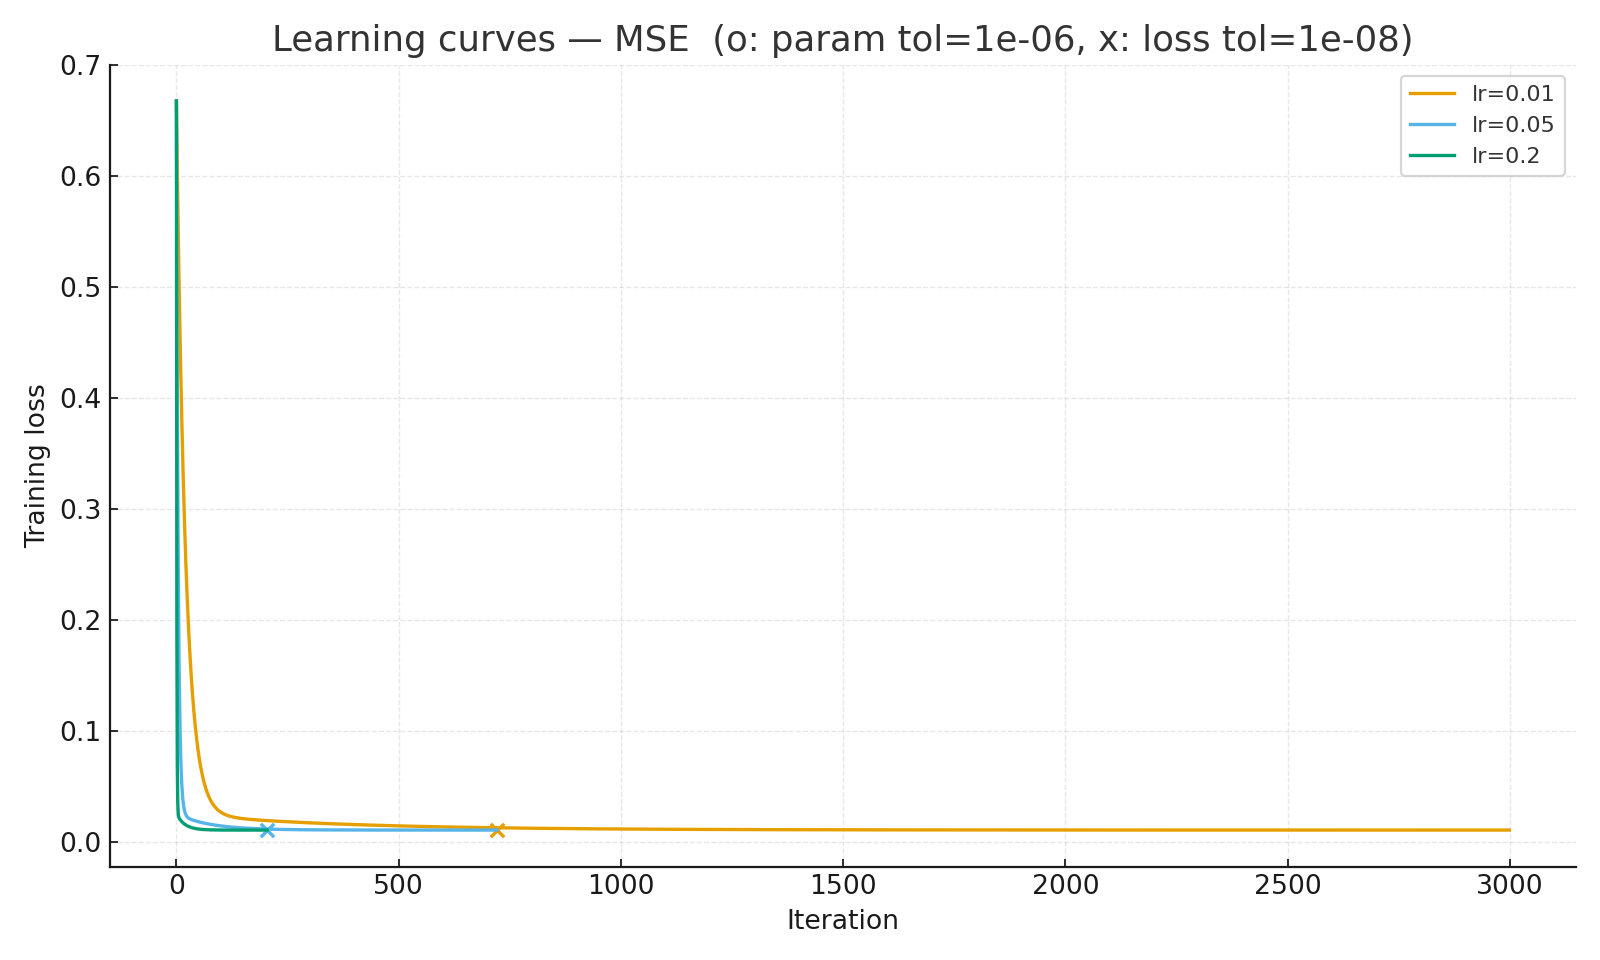
\includegraphics[width=0.9\linewidth]{mse_learning_curves.png}
\caption{Learning curves---MSE \; (o: param tol, x: loss tol). For $\eta{=}0.2$, loss-tol (×) occurs before param-tol (○).}
\label{fig:mse}
\end{figure}

\begin{figure}[H]
\centering
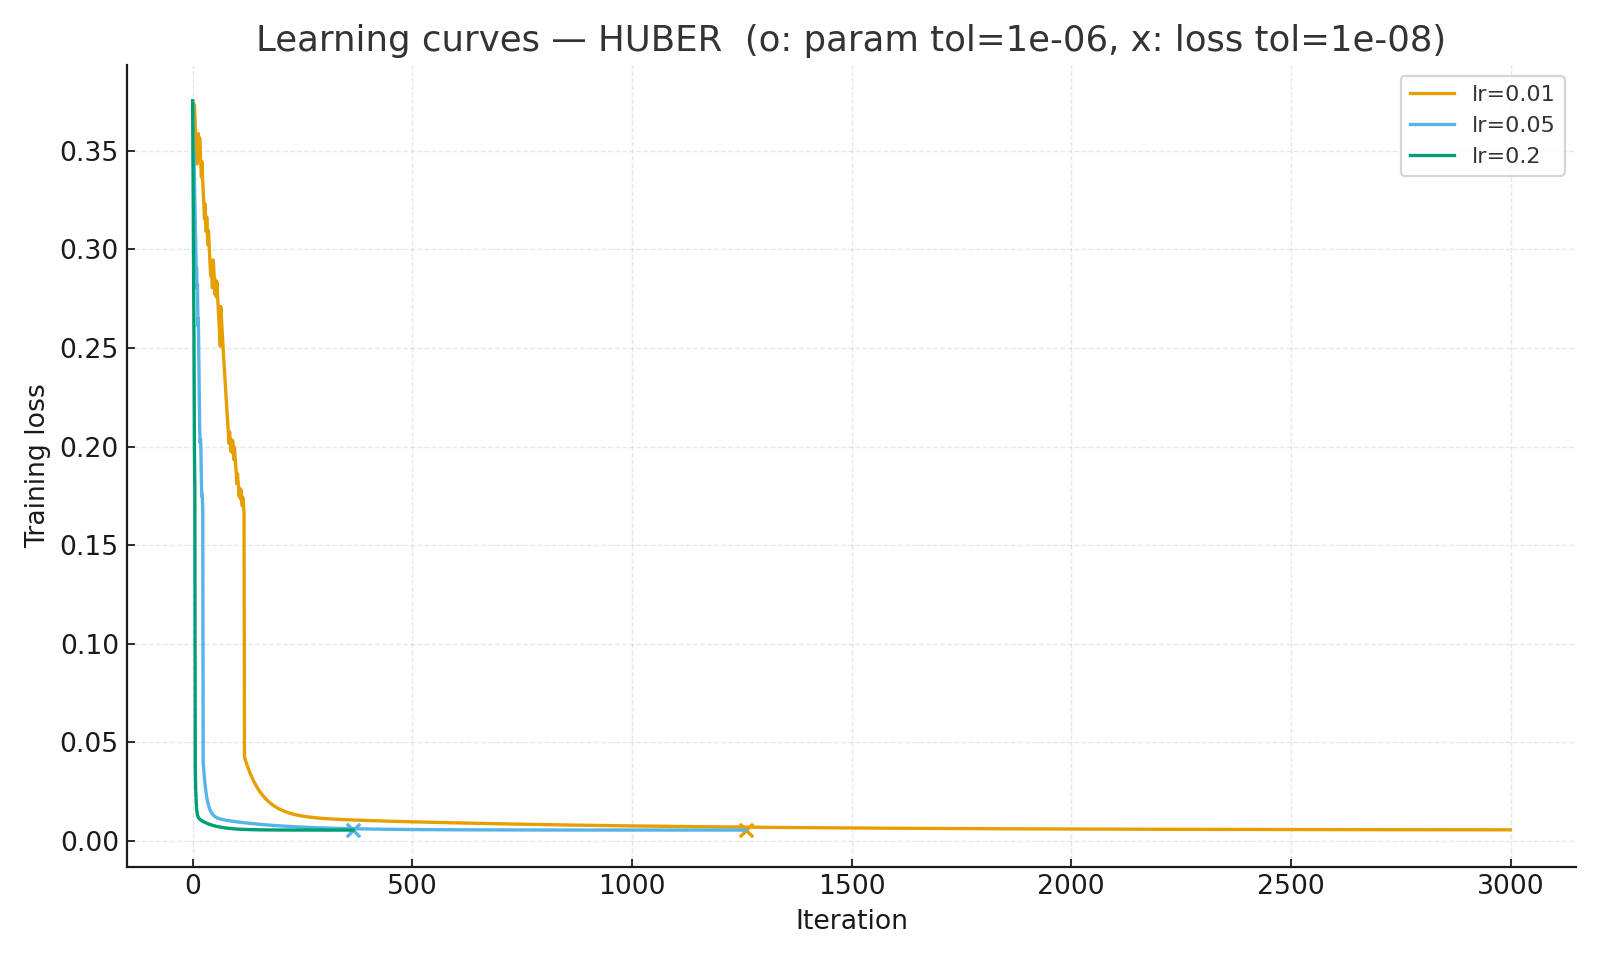
\includegraphics[width=0.9\linewidth]{huber_learning_curves.png}
\caption{Learning curves---Huber \; (o: param tol, x: loss tol). For $\eta{=}0.2$, loss-tol (×) occurs before param-tol (○).}
\label{fig:huber}
\end{figure}

\section{Discussion}
\begin{itemize}[leftmargin=1.5em]
\item \textbf{Effect of learning rate.} Larger $\eta$ substantially reduces iteration count. For both losses, $\eta=0.2$ converged fastest; $\eta=0.01$ was slow and hit the max-iteration cap.
\item \textbf{Stop criteria.} In this run, \emph{both} criteria were reached for $\eta\in\{0.05,0.2\}$. The \emph{loss} tolerance triggered earlier (721/204 iterations for MSE; 1259/365 for Huber), and the \emph{parameter} tolerance triggered later (1172/340 for MSE; 2162/639 for Huber), indicating the objective flattened before the parameters fully stabilized.
\item \textbf{MSE vs.\ Huber.} Huber achieved a slightly lower training loss and shows smooth early-iteration behavior at larger $\eta$, consistent with robustness to outliers.
\item \textbf{Correctness.} GD(MSE) parameters closely match least squares, with $\|\theta_{\mathrm{GD}}-\theta_{\mathrm{LS}}\|_2\approx 1.44\times10^{-4}$.
\end{itemize}
\noindent \textit{Learning-rate taxonomy:} $\eta{=}0.01$ (conservative/slow), $\eta{=}0.05$ (efficient), $\eta{=}0.2$ (aggressive but stable on this dataset).

\section{Reproducibility and Code}
Code, notebook, and figures are available at:\\[2pt]
\textbf{GitHub:} \href{https://github.com/Jay-Sonawane2712000/EEE_511_1233750832_HW_1}{https://github.com/Jay-Sonawane2712000/EEE\_511\_1233750832\_HW\_1}\\[3pt]
To run: \texttt{pip install -r requirements.txt} and execute the notebook or script to produce Figures~\ref{fig:mse}--\ref{fig:huber} and the tables above.

\section*{Conclusion}
GD converges reliably for both MSE and Huber on the provided dataset. Higher learning rates reduce iteration counts without overshooting here, while the Huber loss yields slightly better fit under potential outliers. The agreement with least-squares verifies the implementation.

\end{document}

